\documentclass[a4paper, 11pt]{article}
\usepackage[T1]{fontenc}
\usepackage[utf8]{inputenc}
\usepackage{lmodern}
\usepackage{textcomp}
\usepackage{lastpage}
\usepackage{graphicx}
\usepackage{siunitx}
\usepackage{minted}
\usepackage{lipsum} 
\usepackage{float}
\usepackage[T1]{fontenc}
\usepackage{caption}
\usepackage{subcaption}
\renewcommand*\familydefault{\sfdefault} %% Only if the base font of the document is to be sans serif



\usepackage{fullpage}

\begin{document}
\normalsize
\noindent
\large\textbf{Diamond Light Source Ltd} \hfill\large\textbf{Date: \today}
\\\normalsize Beam Diagnostics Group \hfill Daniel Harryman\\
\centering\\
\section*{}
\vspace{5mm}
\huge\textbf{BPM Test Framework Design \& Operation Report}
\vspace{5mm}
\includegraphics[width = 1\textwidth]{Logo.PNG}
\includegraphics[width = 1\textwidth]{SimpleHW.jpg}
\normalsize
\clearpage
\tableofcontents
\listoffigures
\raggedright
\clearpage
\section{Introduction}
This document details the objectives, design, and implementation of the Beam Position Monitor test framework developed for use at Diamond Light Source, primarily using scripts, that are written in Python. The tests described in this manual will be for testing the electronic readout devices used to analyse the signals that would typically come from physical BPMs (such as button BPM's). A simple test set-up that is used for many tests can be seen in figure \ref{fig:setup}. For this type of test there is a single output source that goes through an equal four way splitter, into the DUT's (Device Under Test's) four inputs, A, B, C, D. It's worth noting that some more advanced tests may require the use of additional hardware that is not shown in figure \ref{fig:setup} and thus will require a different setup. 

\begin{figure}[H]
	\centering
	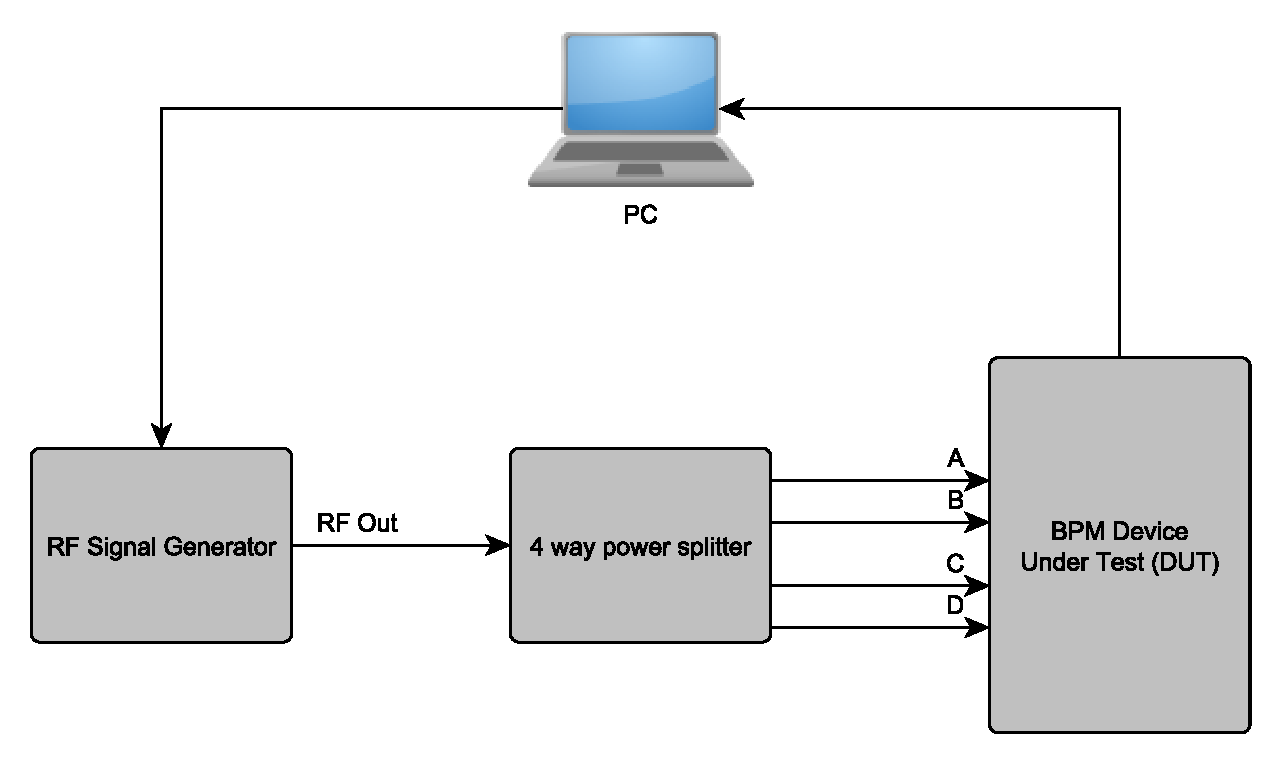
\includegraphics[width=0.8\textwidth]{SimpleSetup.pdf}
	\caption{Simple test setup}
    \label{fig:setup}
\end{figure}

The exact method or protocol used by the PC to communicate with both the RF Signal Generator, and BPM Device Under Test (DUT) may change depending on what hardware models are used. The framework this software uses will abstract such layers away from the final user as much as is possible, making a final product that is both scalable and maintainable.  

\subsection{Objectives}\label{sec:objectives}
The final product or program produced has a specific set of objectives and goals. The task is not only to create a test application, but to ensure the application created can be added to and extended over time, allowing for the supported hardware, and the tests that can be run to grow. 
\begin{itemize}
  \item Create an application or program that will perform tests on the Beam Position Monitor readout instruments, that are used at Diamond. 
  \item Ensure that the hardware is abstracted from the tests, so that the process of changing the hardware used in the tests will not require any of the tests to be rewritten. 
  \item Scalable, the final program must be scalable so that new tests can be added and amended easily, as well as making it easy to run a subset of tests or change the order that the tests are run.
  \item Once a set of tests has run, this should produce a report, that will show the results of the tests. 
  \item The software should be designed to good practices and use appropriate commenting styles, unit testing, and simulation where possible. 
    
\end{itemize}
\section{Software Architecture}\label{sec:SoftwareArchitecture}
Given the objectives stated in section \ref{sec:objectives} the software architecture used must be well designed and thought out. This section of the report details the generic software architecture that has been used to achieve these objectives.  

\subsection{Software Design}
When making a series of tests typically a scripting language will be used. The two most popular ones used in Diamond are \textsc{Matlab} and Python. Python has been chosen as it lends itself to object oriented programing slightly more than \textsc{Matlab}, and it's open source so the final program can be easily ported to a different machine. \\

The main building blocks of the program are the tests, the hardware, and the report. As such a typical test will be a script that has an object for each hardware device, and another for the report that the data will be saved to. Figure \ref{fig:TestAggregation} shows this, the arguments for each test will be an instance of each of the classes shown in the figure \ref{fig:TestAggregation} as well as the test parameters themselves. If more hardware devices are needed, then that will also need to be an object that is used in the test's arguments. \\

\begin{figure}[H]
	\centering
	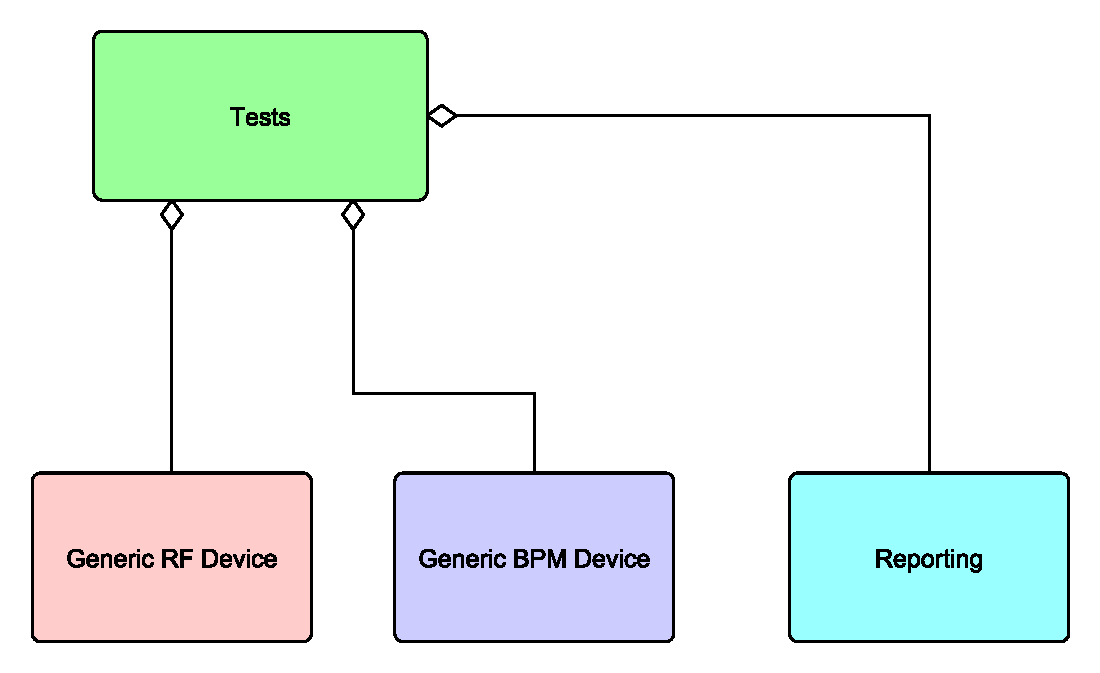
\includegraphics[width=0.6\textwidth]{TestDependency.pdf}
	\caption{Test Aggregation}
    \label{fig:TestAggregation}
\end{figure}

The main script will instantiate all of the objects that are to be called by the tests, then uses these objects as inputs to the relevant test scripts. Figure \ref{fig:launcher.py} shows an example of the main launcher script. This instantiates an object of each of the type of hardware and a report, before feeding into three separate test scripts where the tests are carried out and there results recorded to the report. If the amount, or type of tests were wanted to be changed, the test scripts called by this are simply added, removed, or have their arguments changed.  

\begin{figure}[H]
\begin{minted}[mathescape,linenos,numbersep=1pt,frame=lines,framesep=1mm]{python}
import RFSignalGenerators
import BPMDevice
import Tests
import Latex_Report

# Creates an instance of the RF object to be used in the tests
RF = RFSignalGenerators.Rigol3030DSG_RFSigGen("172.23.252.51", 5555, 1)

# Creates an instance of the BPM object to be used in the tests
BPM = BPMDevice.Libera_BPMDevice(4)

# RF Frequency of Diamond in MHz 
dls_RF = 499.6817682

# Creates the Report object that the results will be saved to
report = Latex_Report.Test_Report("BPM Test Report")

# Performs three different tests by calling three different scripts
Tests.Beam_Current_vs_X_and_Y_Position(RF, BPM, dls_RF, -100, 0, 100, 1, report)
Tests.Input_Power_vs_Beam_Current(RF, BPM, dls_RF, -100, 0, 100, 1, report)
Tests.Output_Power_vs_Input_Power(RF, BPM, dls_RF, -100, 0, 100, 1, report)

# Complies the output report 
report.create_report()
\end{minted}
\caption{Python Test launcher}
\label{fig:launcher.py}
\end{figure}

\subsection{Hardware Abstraction}
Figure \ref{fig:launcher.py} shows how one calls different tests with specific hardware instances. What would happen if a different piece of hardware was to be used instead? In keeping with the objectives given in section \ref{sec:objectives} the ideal solution would require no changes to the code used in the test scripts. This can easily be achieved using an object oriented approach. Generic classes of each hardware type are setup with specific API methods. The children of the generic objects then overload these methods that are called by the test. Figure \ref{fig:HardwareAbstraction} shows an expanded view of figure \ref{fig:TestAggregation}, the tests are still given an instance of each piece of hardware, but as long as the children of the generic objects use the same APIs then the tests will still work. 

\begin{figure}[H]%
	\centering%
	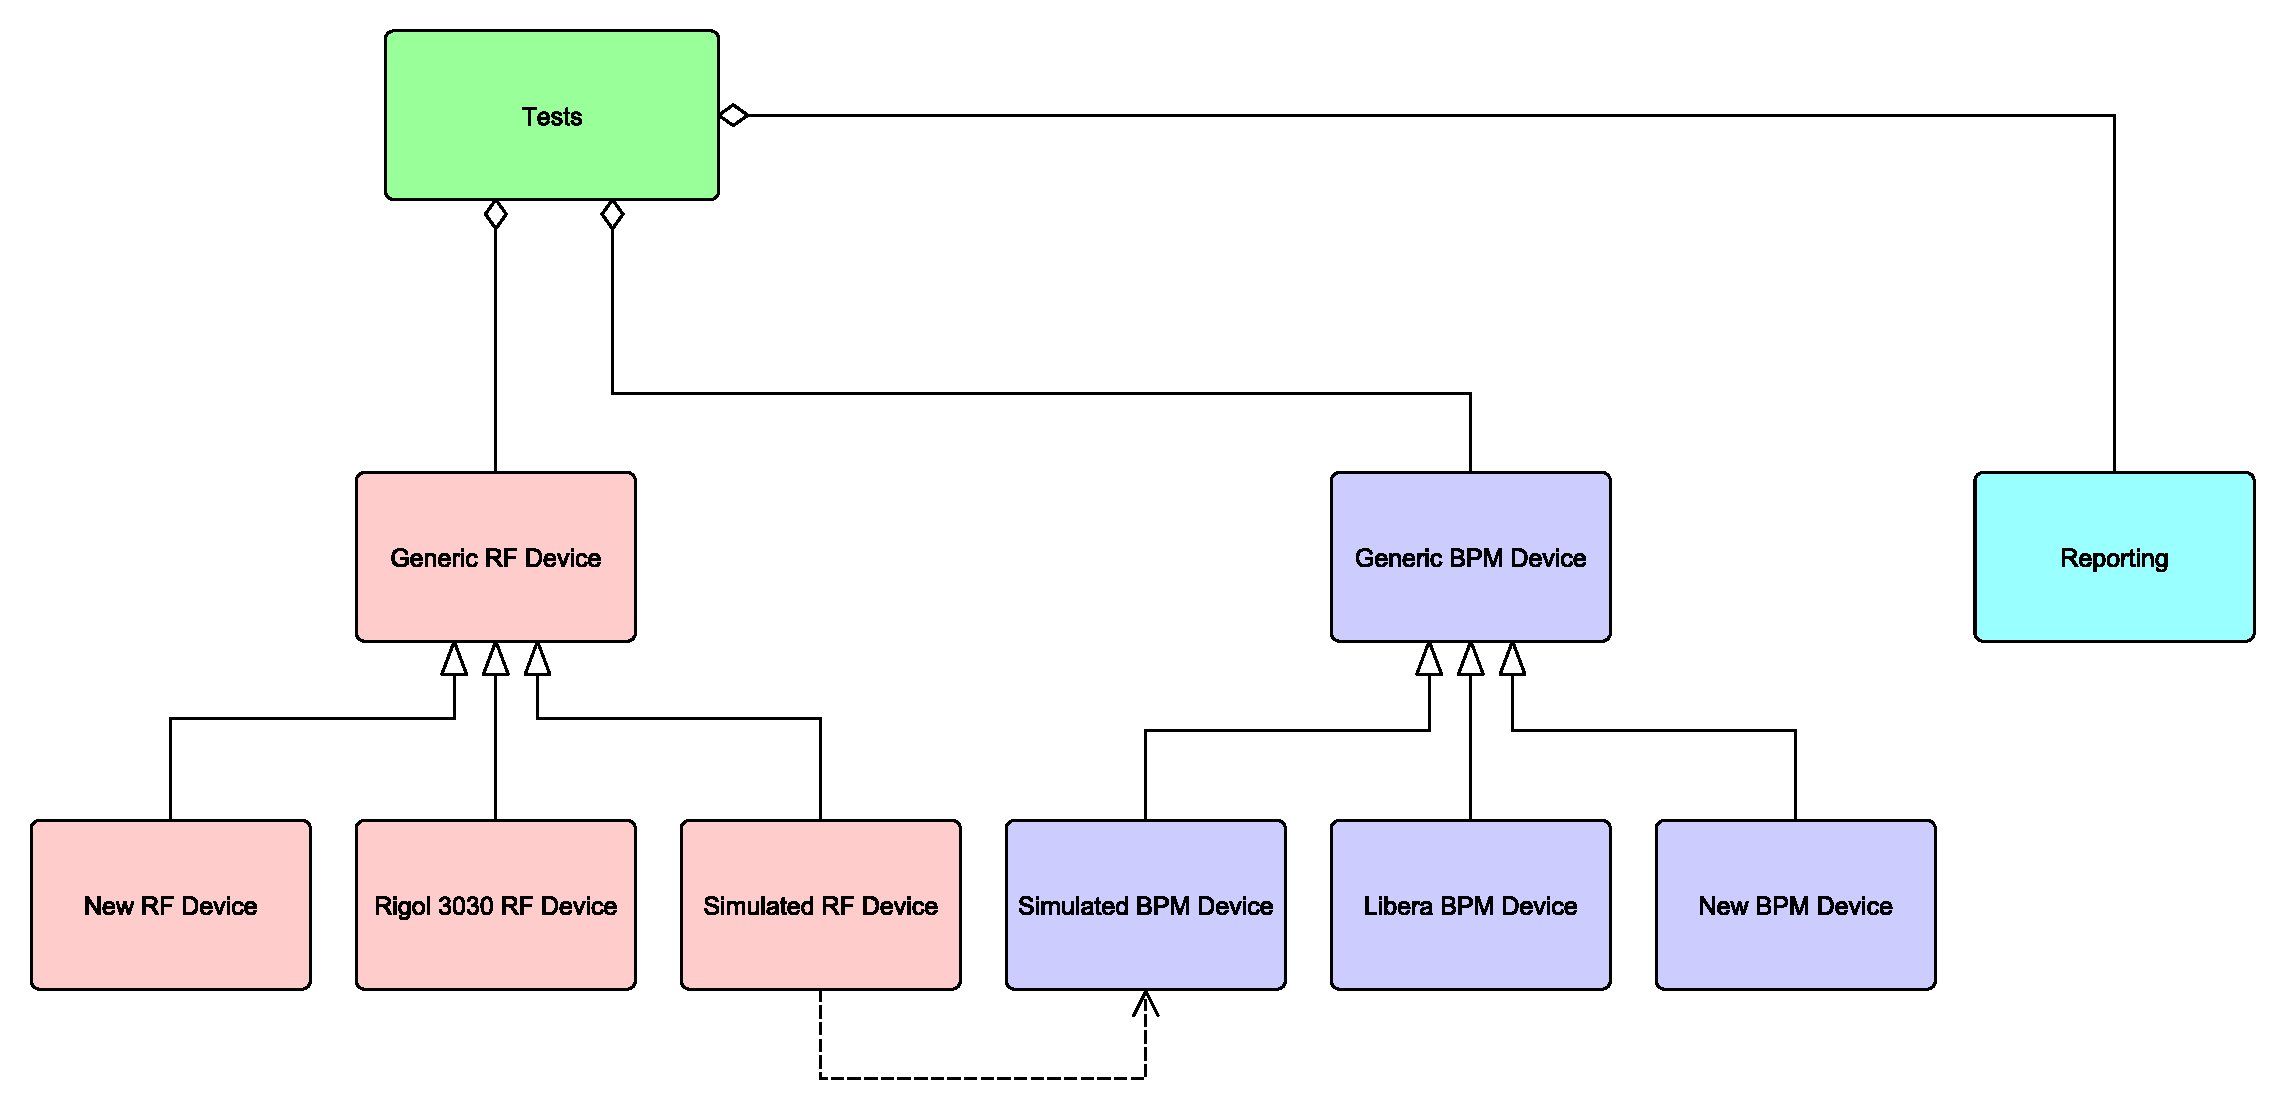
\includegraphics[width=1\textwidth]{HardwareAbstraction.pdf}%
	\caption{Hardware Abstraction Using Classes}%
    \label{fig:HardwareAbstraction}
\end{figure}
Shown in figure \ref{fig:HardwareAbstraction} the \textbf{Simulated BPM device} has a dependency on the \textbf{Simulated RF Device}, this is because there is no physical connection in the real world connecting the output signals from the RF hardware to the BPM hardware, so this is done in software instead with the simulators. 
To the test script, is doesn't matter if the exact implementation of communicating with the RF device is done over Telnet, USB, or a different standard, as that is done in the specific API implementation, and abstracted away from the test. Figure \ref{fig:abstraction.py} shows the implementation of the same function in three different classes, one is the generic parent, one is a simulated version of RF hardware, and the third is the one that communicated with the Rigol 3030 device. Notice how the generic method is decorated with the \textbf{@abstractmethod} decorator. This means that instantiating an object with this method is not possible and will result in an error, these methods \textbf{must} be over ridden by it's child classes. For the simulator class, it simply feeds out it's device ID that is constructed when the object is. For the Rigol 3030 however a Telnet call is made to a physical device with the \textbf{*IDN?} command, the reply is then returned as the device ID. Notice that for each of the methods the name, and arguments are the exact same, this is required on all of the over-ridden methods, and it is good practice to do the same for the return type as well.  This means using one piece of hardware, or another, or a simulator, will only require a change in the instantiation of the object, all of the code in the tests will remain the same. 


\begin{figure}[H]
\begin{minted}[mathescape,linenos,numbersep=1pt,frame=lines,framesep=1mm]{python}
# Generic RF Device Class
@abstractmethod
def get_device_ID(self):
	pass
\end{minted}
\begin{minted}[mathescape,linenos,numbersep=1pt,frame=lines, framesep=1mm]{python}
# Simulated RF Device Class, inherits from "Generic RF Device Class" 
def get_device_ID(self):
	return self.DeviceID
\end{minted}
\begin{minted}[mathescape,linenos, numbersep=1pt,frame=lines,framesep=1mm]{python}
# Rigol 3030 Device Class, inherits from "Generic RF Device Class" 
def get_device_ID(self):
	self.DeviceID = self._telnet_query("*IDN?")
	return self.DeviceID
\end{minted}
\caption{Python Hardware Abstraction}
\label{fig:abstraction.py}
\end{figure}

\subsection{Unit Testing \& Simulation}
Unit testing has been used to test individual class methods, where as system tests are done using simulator classes. For the unit tests the calls to the hardware are mocked out and only the methods functionality is tested. This normally includes checking that the function is called, and that given specific arguments the correct values come back. For example, when setting the output frequency of the RF device, a numeric could be used as the input argument that would assume a default value of \SI{}{\mega\hertz} for the units, or a string could be used that would that specifically states different units, such as \SI{}{\kilo\hertz}. Unit testing is done to ensure that despite the form that the input arguments take, the output is still formatted correctly. \\
Simulation is done to check one of the test scripts quickly and reliably. Simulation can be used to ensure that the plotting and reporting functionality of the tests work as desired without actually needing to connect the hardware. Communication with the hardware is slower than that with a virtual device meaning code iterations can be made much faster, and as long as the simulation is not changed, the results will be fixed for the same set of input arguments.

\section{Software Implementation}
As listed throughout section \ref{sec:SoftwareArchitecture}, the software is implemented in python, with test scripts that call objects that interface with different hardware components. In this section is the specific API and test setup, with some details about their implementation. 

\subsection{Radio Frequency Devices}
As already stated, the \textbf{Generic\_RFSigGen} parent class will set out most of the APIs that can be used to program the device. The name of the APIs are descriptive of their functionality. For example \textbf{set\_frequency(frequency)} will change the frequency output by the RF instrument. Given the method names it's easy to see what their functionality would be, but there are detailed docstrings for all of the APIs and their classes, that should answer questions about functionality. \\
The \textbf{Rigol3030DSG\_RFSigGen} class is a child of \textbf{Generic\_RFSigGen} that communicates using Telnet, as there is a Telnet library for python this takes care of much of the programming required, but the generic Telnet calls are still wrapped in pseudo private methods that are then called by the API methods. The \textbf{\_\_init\_\_} methods are specifically not overridden in the children as the constructors of each class will be different, for the example of the Rigol 3030 the IP address and Port number are used as arguments, whereas if an RS232 instrument was used a COM Port would need to be listed instead. 

\subsection{Beam Position Monitor Devices}
On the initial outset the devices under test are all Libera BPM instruments that communicate using EPICS. As such most of the BPM APIs can easily be implemented using process variables and \textbf{caget} calls. As not all of these BPM instruments are the exact same there is the ability to extend their functionality by creating a child to the \textbf{Libera\_BPMDevice Class}, or by creating a sibling if the functionality is dramatically different. A sibling could also be created to communicate with a BPM instrument that does not use the EPICS protocol. Like the rest of the program if extended information on the exact implementation of the BPM classes and their methods are needed the relevant docstrings should provide it. 

\subsection{Automated Reporting}
Automatic reporting is done using pylatex. This is a python library that will generate and compile a \LaTeX \space report. The methods for the report simplify down to only a few APIs, all of which are shown in figure \ref{fig:TestReportAPIs}. When the \textbf{Test\_Report} object is created it essentially created a single Tex document. Each test will then use the \textbf{setup\_test} method to create a new section in the report for that test, This section will then have a description to the test, that is copied verbatim from the \textbf{introduction\_text} argument. The \textbf{device\_names} expects a list of strings, one for list item for each piece of hardware, typically, this is compiled by running the \textbf{get\_device\_ID} method of each device. The final argument for the \textbf{setup\_test} API is the parameter names, this is also a list of strings, but the strings contain the name of each parameter and  their value, this data is then written to the report. The \textbf{add\_figure\_to\_test} API is called to load a graph from the test into the active section of the report. Finally after all of the tests have been run, the \LaTeX \space report is compiled by the \textbf{create\_report} method. 

\begin{figure}[H]
\begin{minted}[mathescape,linenos,numbersep=5pt,frame=lines,framesep=2mm]{python}
# Class used to create a LaTeX test report
class Test_Report():
  # Set the file name and initialise the report 
  def __init__(self, fname):
  # Create a new section in the report, write the devices and parameters used to it
  def setup_test(self, section_title, introduction_text ,device_names, parameter_names):
  # Add a figure/graph to the current test section
  def add_figure_to_test(self,image_name, caption=""):
  # Compile the LaTeX report and generate an output file
  def create_report(self):
\end{minted}
\caption{Test Report APIs}
\label{fig:TestReportAPIs}
\end{figure}

\subsection{Test Design}
Each test will be a single script that will test a specific parameter, some of these tests may only work with some hardware devices that have advanced features, and as such each test should be as simple as possible allowing for a modular approach when performing the tests. 
\subsubsection{Power Ramp Tests}
Several of the tests can be done by ramping the output power on an RF device and reading different parameter(s) off of the BPM. The \textbf{Beam\_Current\_vs\_X\_and\_Y\_Position} is such a test. A fixed frequency is output and then power output level from the RF device is linearly ramped up as the beam current is recorded along with the X and Y positions of the beam. Figure \ref{fig:BeamCurrentVsXYArguments.py} shows the doc string for the test. This describes the test operation and describes all of the arguments for the test. 

\begin{figure}[H]
\begin{minted}[mathescape,linenos,numbersep=1pt,frame=lines,framesep=1mm]{python}
"""Tests the relationship between beam current and X Y position read from the BPM.

An RF signal is output and then read back using the RF and BPM objects respectively. 
The signal is ramped up in power at a single frequency. The number of samples to take, 
and settling time between each measurement can be decided using the arguments. 
Args:
    RF (RFSignalGenerator Obj): RF interface object.
    BPM (BPMDevice Obj): BPM interface object.
    frequency (float/str): Output frequency for the tests, can be a float, where 
        the units will default to MHz, or can be a string where the units can be 
        explicitly stated e.g. kHz, Hz.
    start_power (float/str): Starting output power for the tests, default value is 
        -100 dBm. The input values can be floats, if so, the units will default to 
        dBm. A string input can be used to explicitly state the units, e.g. dBW, mV.
    end_power (float/str): Final output power for the tests, default value is 0 dBm.
        The input values can be floats, if so, the units will default to dBm. A 
        string input can be used to explicitly state the units, e.g. dBW, mV.
    samples (int): Number of samples taken is this value + 1.
    settling_time (float): Time in seconds, that the program will wait in between 
        setting an  output power, and reading an input power. 
    report (LaTeX Report Obj): Specific report that the test results will be recorded 
        to. If no report is sent to the test then it will just display the results in 
        a graph.
Returns:
    float array: Beam current values during the test. 
    float array: Horizontal position of the BPM during the test.
    float array: Vertical position of the BPM  during the test.
"""
\end{minted}
\caption{Beam\_Current\_vs\_X\_and\_Y\_Position.py Docstring}
\label{fig:BeamCurrentVsXYArguments.py}
\end{figure}

Figure \ref{fig:BeamCurrentVsXY.py} shows a cut down version of the test script, the reporting features, docstrings, and import lines, have been removed. It can be seen, that the main part of the test is performed in lines 18-23. This is just a simple \textbf{for loop} that will record the desired parameters, then step up the output power, wait for the output to settle, then repeat the process again. This is the same process for all of the tests that ramp up the output power. The only difference is that different parameters are recorded and thus the plotting and report writing is different as well.  

\begin{figure}[H]
\begin{minted}[mathescape,linenos,numbersep=1pt,frame=lines,framesep=1mm]{python}
def Beam_Current_vs_X_and_Y_Position(RF,
                                     BPM,
                                     frequency,
                                     start_power=-100,
                                     end_power=0,
                                     samples=10,
                                     settling_time=1,
                                     report=None):
                                     
# Set the initial state of the RF device
power = np.linspace(start_power, end_power, samples) # Creates samples to test
RF.set_frequency(frequency)
RF.set_output_power(start_power)
RF.turn_on_RF()
time.sleep(settling_time)

# Perform the test
for index in power:
  beam_current = np.append(beam_current, BPM.get_beam_current()) # record beam current
  X_pos = np.append(X_pos, BPM.get_X_position()) # record X pos
  Y_pos = np.append(Y_pos, BPM.get_Y_position()) # record Y pos
  RF.set_output_power(index) # Set next output power value
  time.sleep(settling_time) # Wait for signal to settle
 
RF.turn_off_RF()
\end{minted}
\caption{Beam\_Current\_vs\_X\_and\_Y\_Position.py Script}
\label{fig:BeamCurrentVsXY.py}
\end{figure}


\section{Operation Guide}
To simply use the application program only one script needs to be configured, and that is the \textbf{Launcher.py} script. The tests and hardware are then selected using from the classes and tests that have been built for the application. This section will go through a simple setup guide of how to setup such tests and the associated hardware. 

\subsection{Setup for beam current dependence using Rigol 3030 and Libera BPM}
If the desire was to use the Rigol 3030 to output signals, that will test the horizontal and vertical beam current dependence, this section will show how to setup the equipment and script to do just that. The hardware requires feeding an equally split RF signal from the Rigol to the Libera. Both the Libera and the Rigol then communicate over the network to the computer running the tests. The connection is shown in figure \ref{fig:SimpleHW}, The Rigol is on the left of figure \ref{fig:SimpleHW} and the Libera on the right, they are connected from the RF output to the four Libera inputs via an SMA cable and a four way splitter from Mini-Circuits. Both are then connected to the same network as the computer running the tests, ensuring that all the normal caveats regarding IP addresses and subnets are taken into account. 

\begin{figure}[H]
\centering
\includegraphics[width=0.8\textwidth]{SimpleHW.jpg}
\caption{Hardware Setup for Libera Testing}
\label{fig:SimpleHW}
\end{figure}

Once the hardware is connected it is the role of creating or amending the Launcher script. The Launcher sits in the top level of the project hierarchy with all of the tests and classes sitting in relevant sub folders. Figure \ref{fig:ProjectHierarchy} shows an image of the project hierarchy. 

\begin{figure}[H]
\centering
\includegraphics[width=0.7\textwidth]{ProjectStructure.jpeg}
\caption{Project Hierarchy}
\label{fig:ProjectHierarchy}
\end{figure}

The launcher file shown in figure \ref{fig:SplitLauncher.py} shows a split up version of the file. The first part shows how the launcher accesses all of the other scripts and files, this is by importing the four subdirectories. Then the hardware used needs to be instantiated, for this test the Rigol will be done first. The Rigol communicates using Telnet, so it needs an IP address, a port number, and a timeout in seconds, all of these are given as arguments when instantiating the Rigol 3030. The next section instantiates the Libera BPM object, each of these devices has their own ID number to ensure that correct devices process variables are read, the device used in this test has the ID of \textbf{4}.\\ 
The fourth part of figure \ref{fig:SplitLauncher.py} configures the report object that will save and display the output data at the end of the test, it's only argument is setting what the report will be called. Next is the point where all of the Test scripts are called, in this example only the \textbf{Beam\_Current\_vs\_X\_and\_Y\_Position} test is run. The arguments for this test are stated in it's doc string and can be configured as desired, but what is important is that the three objects just instantiated are given as inputs to this object, so they are the ones used in the test. Finally after all of the tests are run, the report is compiled with the \textbf{create\_report} method. 

\begin{figure}[H]
\begin{minted}[mathescape,linenos,numbersep=1pt,frame=lines,framesep=1mm]{python}
# Import sub directories
import RFSignalGenerators
import BPMDevice
import Tests
import Latex_Report
\end{minted}
\begin{minted}[mathescape,linenos,numbersep=1pt,frame=lines,framesep=1mm]{python}
# Instantiate Rigol 3030 Object
RF = RFSignalGenerators.Rigol3030DSG_RFSigGen("172.23.252.51", 5555, 1)
\end{minted}
\begin{minted}[mathescape,linenos,numbersep=1pt,frame=lines,framesep=1mm]{python}
# Instantiate Libera BPM Object
BPM = BPMDevice.Libera_BPMDevice(4)
\end{minted}
\begin{minted}[mathescape,linenos,numbersep=1pt,frame=lines,framesep=1mm]{python}
# Instantiate LaTeX Report Object
report = Latex_Report.Test_Report("BPM Test Report")
\end{minted}
\begin{minted}[mathescape,linenos,numbersep=1pt,frame=lines,framesep=1mm]{python}
# Perform test with given Objects and arguments
dls_RF = 499.6817682 # RF Frequency of Diamond in MHz
power_final = 0 # Final output power of the RF device in dBm
power_start = -100 # Starting output power of the RF device in dBm
samples = 100 # Samples to be taken in the test
settling_time = 2 # Amount of time the 

Tests.Beam_Current_vs_X_and_Y_Position(RF, 
					BPM, 
                                        dls_RF,
                                        power_start, 
                                        power_final, 
                                        samples,
                                        time, 
                                        report)
\end{minted}
\begin{minted}[mathescape,linenos,numbersep=1pt,frame=lines,framesep=1mm]{python}
# Compile final report 
report.create_report()
\end{minted}
\caption{Sectioned Launcher.py script}
\label{fig:SplitLauncher.py}
\end{figure}

When running the script in figure \ref{fig:SplitLauncher.py} a .pdf report will be produced, each test run will append a new section onto the report. The section appended when running the script in figure \ref{fig:SplitLauncher.py} can be seen in figure \ref{fig:ReportOut}. If multiple tests were run, there would just more more sections added to the end of this document with the same details as seen in figure \ref{fig:ReportOut}. 

\begin{figure}[H]
\centering
\fbox{\includegraphics[width=1\textwidth]{reportoutput.pdf}}
\caption{Report page produced from\_Beam\_Current\_vs\_X\_and\_Y\_Position.py}
\label{fig:ReportOut}
\end{figure}
\clearpage
 
\section{How to...}
As mentioned before the program is designed to be scalable. This section will detail a step by step guide on how to extend the tests and also add new hardware devices. The process of adding a new device that has an abstract class is similar for any type of hardware so this is only described once. Some tests may require specialist hardware, as such they will be added without inheriting from an existing class. 

\subsection{Add a new child device with hardware abstraction}
Adding a new child device is made easy by the hardware abstraction layer. If for example a new RF device was to be added the starting point would be to open the \textbf{Template\_RFSigGen.py} file, a version of this file is shown in figure \ref{fig:TemplateRF.py}, the version shown in this figure has the method docstrings removed so it fit in the report easier. As you can see this already has the specific APIs in place ready for the functional code to be added. 

\begin{figure}[H]
\begin{minted}[mathescape,linenos,numbersep=1pt,frame=lines,framesep=1mm]{python}
from Generic_RFSigGen import *

class Template_RFSigGen(Generic_RFSigGen):
    """template, Child of Generic_RFSigGen.

    Attributes:  
        *Inherited from parent.
    """

    # Private Methods go here

    # Constructor and Deconstructor
    def __init__(self):

    def __del__(self):

    # API Calls
    def get_device_ID(self):
	# Code to get device ID goes here
    def get_output_power(self):
	# Code to get output power level goes here
    def get_frequency(self):
    # code the get the current output frequency goes here
    def set_frequency(self, frequency):
	# Code to set the output frequency goes here
    def set_output_power(self, power):
	# Code to set the output power level goes here
    def turn_on_RF(self):
	# Code to enable the RF output goes here
    def turn_off_RF(self):
	# Code to disable the RF output goes here
    def get_output_state(self):
	# Code to check if the RF output is enabled or disabled goes here 
\end{minted}
\caption{Template\_RFSigGen.py}
\label{fig:TemplateRF.py}
\end{figure}

If we wanted to add the AtlanTecRF ASG3000-U instrument to this program this would be the starting point. 
\subsection{Add a new device without hardware abstraction}
When this is required in the development of the product/program a step by step guide will be added here. 
\subsection{Add a new Test}
When the next test is added to the report, a step by step guide of that will be added here. 

\end{document}